\subsection{MVC}
As we said in the introduction we think that the teamwork and the complexity of the project needs a more structured approach, and we found valid guidelines into the \textit{hecodes} blog \cite{mvcarticle}. This section will not provide a useless repetition of the cited article, conversely we'll focus on the differences. 
Due to the complexity of the project if compared to the example we had to make some different design choices, mainly the worhy of note are two:
\begin{itemize}
\item The TurretMediator doesn't directly contain the object3D related to the turret but a container that contains the turret itself plus the bullet, this hierarchy is done just to make the bullet's movement easier to generate.
\item The second difference is about the controller, into the example we have just one controller related with the MainView, in our implementation we had too many function and we created many more controllers, everyone associated with his own mediator. We also decide that Every controller is in charge of every logic operation such as the computation of the next position, even if in the article it has just to react to user inputs.
\end{itemize}
\begin{figure}[h!]
\begin{center}
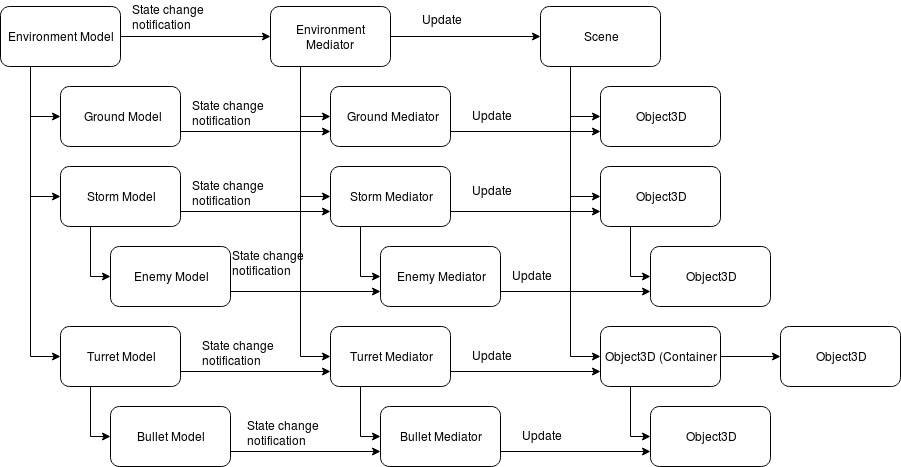
\includegraphics[scale=0.5]{images/MVC.png}
\caption{The structure of the software}
\end{center}
\end{figure}
